\section{IP YÖNLENDİRME}

IP'nin yönlendirilebilir olması protokolün  en güçlü özelliğidir. Çok sayıda iletişim protokolü mevcut olmasına rağmen IP'nin yönlendirilebilir esnek yapısı internetin temel dili olmasını sağlamıştır. Yönlendirme işlemini "Yönlendirici(Router)" yapar.

\textbf{Yönlendirme Tablosunda}
\begin{enumerate}[label=\alph*)] 
   \item Kaynak
   \item Hedef(Ip ve Maske)
   \item Ağ Geçidi
   \item Ara Birim(Interface)
   \item Ölçüt(Metrik)
\end{enumerate}

\begin{figure}[ht]
    \centering
    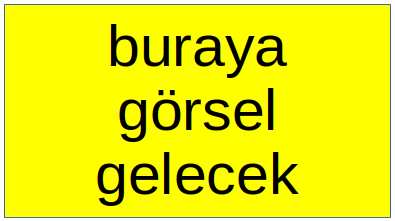
\includegraphics[width=5cm]{images/BurayaGorselGelecek.png}
    \caption{Yönlendirme Tablosu}
    \label{fig:YonlendirmeTablosu}
\end{figure}

\subsection{STATİK YÖNLENDİRME}
Ağ yöneticisi tarafından elle sabit olarak yazılır.Genellikle yönlendiricisi ve yönlendirme işlemi çok fazla olmayan ağlarda kullanılır.Yönlendirme tablolarının güncellemesi ağdaki fiziksel değişikliklere göre yeniden elle yapılmalıdır.

\begin{figure}[ht]
    \centering
    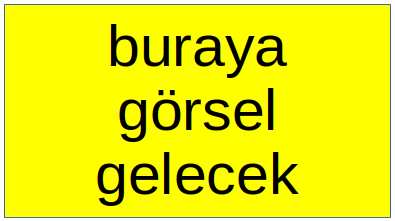
\includegraphics[width=5cm]{images/BurayaGorselGelecek.png}
    \caption{Statik Yönlendirme}
    \label{fig:StatikYonlendirme}
\end{figure}

\subsection{DİNAMİK YÖNLENDİRME}
Yönlendirme algoritmaları  tarafından hesaplanarak bulunur. Ağ yöneticisi tarafından önceden bazı filtreler ve tanımlamalar yapılmalıdır. Ağda değişiklik olduğunda yollar otomatik olarak düzeltilir. En yaygın yönlendirme algoritmadır.

\begin{figure}[ht]
    \centering
    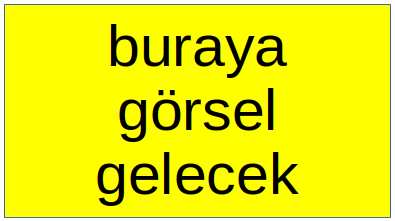
\includegraphics[width=5cm]{images/BurayaGorselGelecek.png}
    \caption{Dinamik Yönlendirme1}
    \label{fig:DinamikYonlendirme1}
\end{figure}

şekildeki ağın sağlıklı çalışabilmesi için  ..... sağlanmalıdır

\begin{figure}[ht]
    \centering
    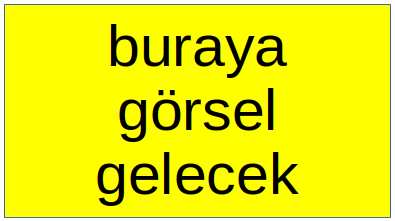
\includegraphics[width=5cm]{images/BurayaGorselGelecek.png}
    \caption{Dinamik Yönlendirme2}
    \label{fig:DinamikYonlendirme2}
\end{figure}

\begin{enumerate}
   \item C'nin E1 bacağı ile A aynı ağda olmalıdır.
   \item  C'nin E2 bacağı ile B aynı ağda olmalıdır.
   \item  A'nin ağ geçidi C'nin E1 bacağındaki IP olmadır.
   \item  B'nın ağ geçidi C'nin E2 bacağındaki IP olmalıdır.
   \item C'ye IP yönlendirme komutu verilmelidir.
\end{enumerate}

Yönlendirme tablosunda birbirini kapsayan kurallar var ise bunlar küçükten büyüğe sıra ie değerlendirilir.

\begin{figure}[ht]
    \centering
    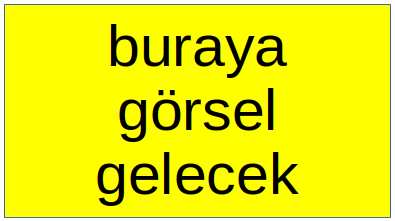
\includegraphics[width=5cm]{images/BurayaGorselGelecek.png}
    \caption{Dinamik Yönlendirme3}
    \label{fig:DinamikYonlendirme3}
\end{figure}

Örnek trafik 10.0.0.5 IP'yi google götürmek üzere /26 kullanır. Gerçi hepsini kapsıyor ondan en küçüğün kabul eder. 10.0.0.199 google göstermek için /24 kullanır.

\begin{figure}[ht]
    \centering
    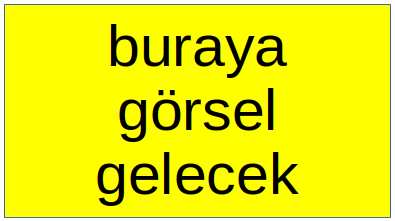
\includegraphics[width=5cm]{images/BurayaGorselGelecek.png}
    \caption{Dinamik Yönlendirme4}
    \label{fig:DinamikYonlendirme4}
\end{figure}

\begin{center}
 \underline{Yönlendirme Tablosu}
\end{center}

\begin{table}[ht]
   \centering  
   \begin{tabular}{llll}
   A $\rightarrow$ B & 10.0.1.0/24 & 10.0.2.0/24 & E2\\
   B $\rightarrow$ A & 10.0.2.0/24 & 10.0.1.0/24 & E1\\
   (A+B)    $\rightarrow$  & 0.0.0.0/0 & 0.0.0.0/0 & E3
  \end{tabular}
  \caption{Tablo XXX}    
\end{table}

\textcolor{red}{NOT: } Yönlendiriciler de kendisine doğrudan bağlıdan (directly connected) ağlar için genellikle yönlendirme  çünkü doğrudan bağlı olan bütün ağlar tanırlar.

\begin{table}[ht]
   \centering
   \begin{tabular}{lll}
   \textcolor{red}{\underline{Directly Connected}}&   
   & \textcolor{red}{\underline{Eklenmesi Gerekenler}}\\
   A$\rightarrow$ 1,2 && A$\rightarrow$ 3,5,b \} 3 satır kural eklemesi gerekiyor\\
   B$\rightarrow$ 2,3,4 && A$\rightarrow$ 1,5,b \} 3 satır\\
   c$\rightarrow$ 1,2 &&A$\rightarrow$ 1,3 \} 2 satır \\
  \end{tabular}
  \caption{Tablo XXX}    
\end{table}
